% Placement and width check only. All text blocks are explicit writing placeholders.
% This is not a draft paper. Manual page breaks are preview aids only.
\documentclass{article}
\usepackage[T1]{fontenc}
% Explicit lowercase font definition avoids a MiKTeX case-lookup fallback here.
\input{t1ptm.fd}
\makeatletter\def\input@path{{sources/neurips2026/}}\makeatother
\usepackage[preprint]{neurips_2026}
\usepackage{graphicx,array,longtable}
\newcommand{\writing}[2]{\par\noindent\fbox{\parbox[c][#1][c]{\dimexpr\linewidth-2\fboxsep-2\fboxrule\relax}{\centering\textbf{WRITING PLACEHOLDER}\par #2}}\par\medskip}
\title{LAYOUT ONLY: AICC5102 paper preparation}
\author{Author names and affiliations placeholder}
\begin{document}
\maketitle
\begin{abstract}
\textbf{WRITING PLACEHOLDER:} problem, extension, scope, two verified findings and final M3 takeaway. No abstract prose has been drafted.
\end{abstract}
\section{Introduction}
\writing{1.4in}{Motivation, one research question, unified contributions.}
\section{Related Work}
\writing{0.9in}{Original paper/code, classical search and verified related work.}
\newpage
\section{Method and Extensions}
\writing{3.0in}{Original pipeline; A*/WA*/IDA*; guarantees; exact references; M3 measurement protocol.}
\section{Experimental Setup}
\writing{2.5in}{Manifest, matched scopes, budgets, hash seeds, metrics and missing references.}
\newpage
\section{Results}
\subsection{Reproduction}
% Generated by paper_preparation/scripts/build_paper_tables_and_figures.py
% Requires array,longtable; place outside table floats. Normal font size.
% CSV is authoritative. Split panels repeat identifying columns.
\begingroup
\setlength{\tabcolsep}{2pt}
\begin{longtable}{>{\raggedright\arraybackslash}p{\dimexpr 0.166667\linewidth-2\tabcolsep\relax}>{\raggedright\arraybackslash}p{\dimexpr 0.166667\linewidth-2\tabcolsep\relax}>{\raggedright\arraybackslash}p{\dimexpr 0.166667\linewidth-2\tabcolsep\relax}>{\raggedright\arraybackslash}p{\dimexpr 0.166667\linewidth-2\tabcolsep\relax}>{\raggedright\arraybackslash}p{\dimexpr 0.166667\linewidth-2\tabcolsep\relax}>{\raggedright\arraybackslash}p{\dimexpr 0.166667\linewidth-2\tabcolsep\relax}}
\hline
Domain & Paper R1/90 & Paper FF/90 & Ours R1/30 & Ours FF/30 & Ours max/30 \\ \hline\endhead
Blocksworld & 66 & 24 & 20 & 8 & 5 \\
Miconic & 90 & 74 & 29 & 20 & 9 \\
Transport & 59 & 29 & 15 & 10 & 5 \\
\hline
\end{longtable}
\endgroup
% Same-machine regeneration: 270 GBFS runs; R1/FF/max = 64/38/19. Paper: 1800 s, 8192 MiB, PyPy; ours: 60 s, 4096 MiB, CPython. Different task counts. Published hmax not reported. Amina's historical 53/25/14 remains a separate, document-only result.

\noindent\textbf{CAPTION PLACEHOLDER:} reduced task counts and budgets; same-machine regeneration distinguished from historical M1.
\writing{0.7in}{Interpret the reproduced ranking and discrepancies.}
\subsection{Search Algorithm Comparison}
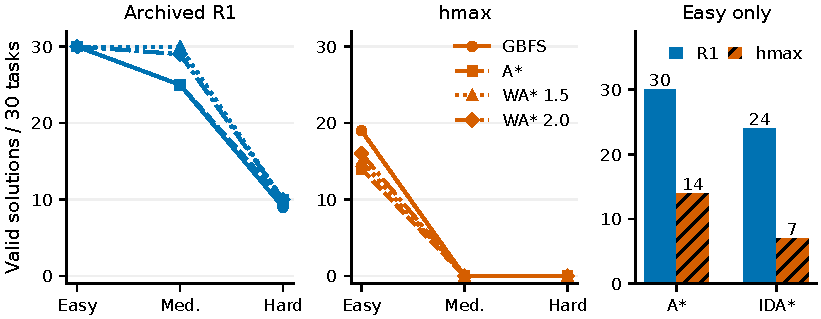
\includegraphics[width=\linewidth]{figures/main/F1_coverage_scaling.pdf}
\noindent\textbf{CAPTION PLACEHOLDER:} 30 tasks/tier; IDA* easy only; budgets and single fixed run.
\writing{0.7in}{Coverage and harder-condition interpretation.}
\newpage
\subsection*{Search comparison continued}
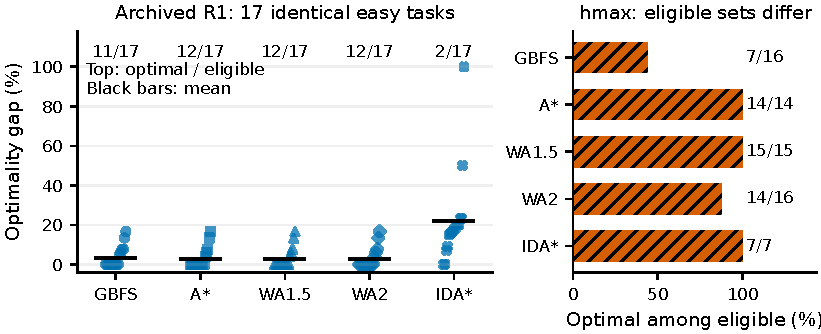
\includegraphics[width=\linewidth]{figures/main/F2_plan_quality.pdf}
\noindent\textbf{CAPTION PLACEHOLDER:} same17 LLM easy-reference tasks; hmax denominators differ; means and optimal counts.
\writing{2.0in}{Quality, matched effort, weighting qualifications and IDA* behavior.}
\subsection{Heuristic Reliability and Robustness}
\writing{0.8in}{Interim initial-state evidence and transition to real M3 results.}
\newpage
\subsection*{Reliability and robustness continued}
\writing{2.3in}{RESERVED MAIN FIGURE: actual R6 accuracy plus R8 trial stability. No data available; no plot invented.}
\noindent\textbf{CAPTION PLACEHOLDER:} actual state/task denominators, three independent trials, SD definition and archived comparator.
\writing{2.3in}{R6--R9 findings or negative results, task-level joins and uncertainty.}
\newpage
\section{Limitations}
\writing{1.3in}{Reference bias; easy-only IDA*; resources; timing and phase uncertainty; trial limits.}
\section{Conclusion}
\writing{0.8in}{Answer the question at the strength supported by final evidence.}
\writing{1.2in}{Reallocate unused preview whitespace to actual preceding sections. References, appendix, contributions and AI-use statement follow the final six main pages.}
\end{document}
